
%% helper macros

\newcommand\pgfmathsinandcos[3]{%
  \pgfmathsetmacro#1{sin(#3)}%
  \pgfmathsetmacro#2{cos(#3)}%
}
\newcommand\LongitudePlane[3][current plane]{%
  \pgfmathsinandcos\sinEl\cosEl{#2} % elevation
  \pgfmathsinandcos\sint\cost{#3} % azimuth
  \tikzset{#1/.estyle={cm={\cost,\sint*\sinEl,0,\cosEl,(0,0)}}}
}
\newcommand\LatitudePlane[3][current plane]{%
  \pgfmathsinandcos\sinEl\cosEl{#2} % elevation
  \pgfmathsinandcos\sint\cost{#3} % latitude
  \pgfmathsetmacro\yshift{\cosEl*\sint}
  \tikzset{#1/.estyle={cm={\cost,0,0,\cost*\sinEl,(0,\yshift)}}} %
}
\newcommand\DrawLongitudeCircle[2][1]{
  \LongitudePlane{\angEl}{#2}
  \tikzset{current plane/.prefix style={scale=#1}}
   % angle of "visibility"
  \pgfmathsetmacro\angVis{atan(sin(#2)*cos(\angEl)/sin(\angEl))} %
  \draw[current plane] (\angVis:1) arc (\angVis:\angVis+180:1);
  \draw[current plane,dashed] (\angVis-180:1) arc (\angVis-180:\angVis:1);
}
\newcommand\DrawLatitudeCircle[2][1]{
  \LatitudePlane{\angEl}{#2}
  \tikzset{current plane/.prefix style={scale=#1}}
  \pgfmathsetmacro\sinVis{sin(#2)/cos(#2)*sin(\angEl)/cos(\angEl)}
  % angle of "visibility"
  \pgfmathsetmacro\angVis{asin(min(1,max(\sinVis,-1)))}
  \draw[current plane] (\angVis:1) arc (\angVis:-\angVis-180:1);
  \draw[current plane,dashed] (180-\angVis:1) arc (180-\angVis:\angVis:1);
}

\begin{tikzpicture}
\tikzstyle{cir} = [draw,line width=0.5pt,align=center,minimum height=0.5em,minimum width=0.5em,circle,fill=white]
\tikzstyle{rec} = [draw,line width=0.5pt,align=center,minimum height=0.5em,minimum width=0.5em,fill=white]
\node[](circle1) at (0,0) {
\begin{tikzpicture} % "THE GLOBE" showcase

\begin{scope}[rotate=30]
\def\R{1.4} % sphere radius
\def\angEl{35} % elevation angle
\filldraw[ball color=gray!20] (0,0) circle (\R);
\foreach \t in {-80,-60,...,80} { \DrawLatitudeCircle[\R]{\t} }
\foreach \t in {-5,-35,...,-175} { \DrawLongitudeCircle[\R]{\t} }
\end{scope}

\end{tikzpicture}
};
\node[](circle2) at ([xshift=3.0em]circle1.east) {
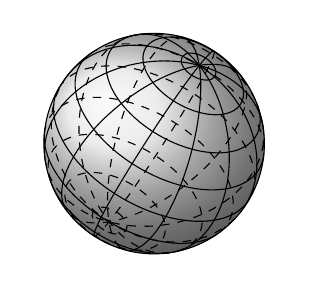
\begin{tikzpicture} % "THE GLOBE" showcase
\begin{scope}[rotate=-30]
\def\R{1.4} % sphere radius
\def\angEl{35} % elevation angle
\filldraw[ball color=gray!20] (0,0) circle (\R);
\foreach \t in {-80,-60,...,80} { \DrawLatitudeCircle[\R]{\t} }
\foreach \t in {-5,-35,...,-175} { \DrawLongitudeCircle[\R]{\t} }
\end{scope}
\end{tikzpicture}
};
\node[](circle3) at ([xshift=5.5em]circle2.east) {
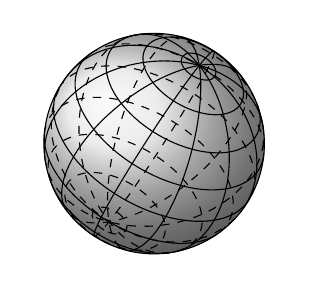
\begin{tikzpicture} % "THE GLOBE" showcase
\begin{scope}[rotate=-30]
\def\R{1.4} % sphere radius
\def\angEl{35} % elevation angle
\filldraw[ball color=gray!20] (0,0) circle (\R);
\foreach \t in {-80,-60,...,80} { \DrawLatitudeCircle[\R]{\t} }
\foreach \t in {-5,-35,...,-175} { \DrawLongitudeCircle[\R]{\t} }
\end{scope}
\end{tikzpicture}
};
\node[](circle4) at ([xshift=5.5em]circle3.east) {
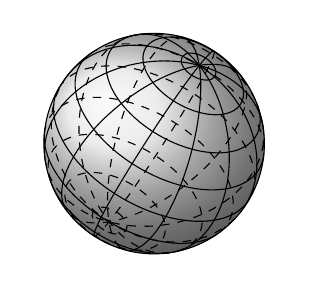
\begin{tikzpicture} % "THE GLOBE" showcase
\begin{scope}[rotate=-30]
\def\R{1.4} % sphere radius
\def\angEl{35} % elevation angle
\filldraw[ball color=gray!20] (0,0) circle (\R);
\foreach \t in {-80,-60,...,80} { \DrawLatitudeCircle[\R]{\t} }
\foreach \t in {-5,-35,...,-175} { \DrawLongitudeCircle[\R]{\t} }
\end{scope}
\end{tikzpicture}
};
\draw[->,very thick] ([xshift=-0.5em]circle2.east)--([xshift=0.5em]circle3.west)node [pos=0.5,above] (pos1) {\scriptsize{$\mathbi{Y}$空间}};
\node [anchor=south](pos1-2) at ([yshift=-0.5em]pos1.north){\scriptsize{\mathbi{X}映射到}};
\draw[->,very thick] ([xshift=-0.5em]circle3.east)--([xshift=0.5em]circle4.west)node [pos=0.5,above] (pos2) {\scriptsize{推断}};
\node [anchor=south](pos2-2) at ([yshift=-0.5em]pos2.north){\scriptsize{词典}};

%circle1
\node[rec,anchor=center,rotate=60,fill=red!20](c1x1) at ([xshift=-7em,yshift=-1.4em]circle1.east){\tiny{1}};
\node[rec,anchor=center,rotate=60,fill=red!20](c1x2) at ([xshift=-4.5em,yshift=1.8em]circle1.east){\tiny{2}};
\node[rec,anchor=center,rotate=60,fill=red!20](c1x3) at ([xshift=-4em,yshift=-0.5em]circle1.east){\tiny{3}};
\node[rec,anchor=center,rotate=60,fill=red!20](c1x4) at ([xshift=-3.5em,yshift=-2.5em]circle1.east){\tiny{4}};
\node[rec,anchor=center,rotate=60,fill=red!20](c1x5) at ([xshift=-2em,yshift=1.0em]circle1.east){\tiny{5}};

%circle2
\node[cir,anchor=center,rotate=-30,fill=blue!20] (c2a) at ([xshift=-5.3em,yshift=2.15em]circle2.east){\tiny{$a$}};
\node[cir,anchor=east,rotate=-30,fill=blue!20] (c2b) at ([xshift=2.0em,yshift=-1.25em]c2a.east){\tiny{$b$}};
\node[cir,anchor=east,rotate=-30,fill=blue!20] (c2c) at ([xshift=0.8em,yshift=-3.9em]c2a.south){\tiny{$c$}};
\node[cir,anchor=east,rotate=-30,fill=blue!20] (c2x) at ([xshift=-0.3em,yshift=-1.9em]c2a.south){\tiny{$x$}};
\node[cir,anchor=west,rotate=-30,fill=blue!20] (c2y) at ([xshift=1.15em,yshift=-2.85em]c2a.east){\tiny{$y$}};

%circle3
\node[rec,anchor=center,rotate=-30,fill=red!20] (c3x1) at ([xshift=-6.7em,yshift=1.75em]circle3.east){\tiny{1}};
\node[rec,anchor=east,rotate=-30,fill=red!20] (c3x2) at ([xshift=4.7em,yshift=-0.95em]c3x1.east){\tiny{2}};
\node[rec,anchor=east,rotate=-30,fill=red!20] (c3x3) at ([xshift=2.6em,yshift=-2.4em]c3x1.south){\tiny{3}};
\node[rec,anchor=east,rotate=-30,fill=red!20] (c3x4) at ([xshift=0.35em,yshift=-2.7em]c3x1.south){\tiny{4}};
\node[rec,anchor=west,rotate=-30,fill=red!20] (c3x5) at ([xshift=2.35em,yshift=-3.85em]c3x1.east){\tiny{5}};

%circle4
\node[rec,anchor=center,rotate=-30,fill=red!20] (c4x1) at ([xshift=-6.7em,yshift=1.75em]circle4.east){\tiny{1}};
\node[rec,anchor=east,rotate=-30,fill=red!20] (c4x2) at ([xshift=4.7em,yshift=-0.95em]c4x1.east){\tiny{2}};
\node[rec,anchor=east,rotate=-30,fill=red!20] (c4x3) at ([xshift=2.6em,yshift=-2.4em]c4x1.south){\tiny{3}};
\node[rec,anchor=east,rotate=-30,fill=red!20] (c4x4) at ([xshift=0.35em,yshift=-2.7em]c4x1.south){\tiny{4}};
\node[rec,anchor=west,rotate=-30,fill=red!20] (c4x5) at ([xshift=2.35em,yshift=-3.85em]c4x1.east){\tiny{5}};

\node[cir,anchor=center,rotate=-30,fill=blue!20] (c4a) at ([xshift=-5.3em,yshift=2.15em]circle4.east){\tiny{$a$}};
\node[cir,anchor=east,rotate=-30,fill=blue!20] (c4b) at ([xshift=2.0em,yshift=-1.25em]c4a.east){\tiny{$b$}};
\node[cir,anchor=east,rotate=-30,fill=blue!20] (c4c) at ([xshift=0.8em,yshift=-3.9em]c4a.south){\tiny{$c$}};
\node[cir,anchor=east,rotate=-30,fill=blue!20] (c4x) at ([xshift=-0.3em,yshift=-1.9em]c4a.south){\tiny{$x$}};
\node[cir,anchor=west,rotate=-30,fill=blue!20] (c4y) at ([xshift=1.15em,yshift=-2.85em]c4a.east){\tiny{$y$}};

\draw [color=red,line width=0.7pt,rotate=18] ([xshift=-5.1em,yshift=3.7em]circle4.east) ellipse (1.6em and 0.9em); 
\draw [color=red,line width=0.7pt,rotate=-5] ([xshift=-2.8em,yshift=0.6em]circle4.east) ellipse (1.6em and 0.9em);
\draw [color=red,line width=0.7pt,rotate=65] ([xshift=-3.10em,yshift=2.10em]circle4.east) ellipse (1.6em and 0.9em);
\draw [color=red,line width=0.7pt,rotate=60] ([xshift=-3.75em,yshift=3.7em]circle4.east) ellipse (1.5em and 0.9em);
\draw [color=red,line width=0.7pt,rotate=65] ([xshift=-3.4em,yshift=5.9em]circle4.east) ellipse (1.5em and 0.9em);

\node [anchor=north](part1) at ([yshift=0.5em]circle1.south){\small{$\mathbi{X}$}};
\node [anchor=west](part2) at ([xshift=6em]part1.east){\small{$\mathbi{Y}$}};
\node [anchor=west](part3) at ([xshift=8.5em]part2.east){\small{$\mathbi{X} \mathbi{W}$}};
\node [anchor=west](part3) at ([xshift=15.0em]part2.east){\small{$\mathbi{X} \mathbi{W}$和$\mathbi{Y}$在同一空间}};

\node [anchor=center](c1) at (5.4,-1.0){\small{$\mathbi{W}$}};

\draw[->,thick] (5.8,-1.2)..controls (5.5,-1.5) and(5.2,-1.2) ..(5.2,-1.2)..controls (4.9,-0.9) and (5.2,-0.6)..(5.5,-0.6);


\end{tikzpicture}
